\documentclass{beamer}

% Solarized Theme
\usecolortheme[light, accent=orange]{solarized}
\beamertemplatenavigationsymbolsempty

\usepackage{graphicx}
\usepackage{hyperref}
\usepackage{booktabs}
\usepackage{amsmath}
\usepackage{diagbox}
\usepackage{tikz}
\usetikzlibrary{calc}

\title{Playing Games}
\author{Michalis Panayides}
\date{}

\begin{document}

\begin{frame}
    \maketitle
    \begin{center}
        
\includegraphics[width=.3\textwidth]{Bin/CUident_CMYK.eps}
    \end{center}
\end{frame}

\begin{frame}
    \begin{center}
        \Large
        What is a game?
    \end{center}
\end{frame}

\begin{frame}
    \centering
    \Large
    \(\frac{2}{3}\)rds of the average game.

    \pause
    \vspace*{2cm}
    \scriptsize
    \underline{\textbf{Rules}}
    \begin{enumerate}
        \item Every player must write a whole number between 0 and 100 on a
        sheet of paper.
        \item The winner of the game will be the player whose number is closest
        to \(\frac{2}{3}\)rds of the average of all the numbers written by all
        the players.
    \end{enumerate}

    \vspace*{1cm}
    \textbf{Example:} There are 3 players who guessed the following numbers:
    \(3, 67 \text{ and } 84\).
    The average would be \(\frac{3 + 67 + 84}{3} = 51.33\).
    The closest guess to \(\frac{2}{3}\) of the average (34.22) is the player
    whose guess was 3.
\end{frame}

\begin{frame}
    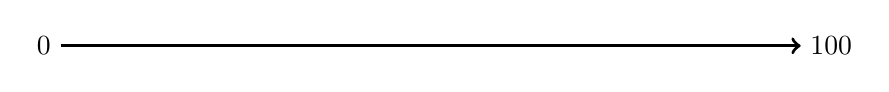
\begin{tikzpicture}
        \node (A) at (0, 0) {0};
        \node (B) at (10, 0) {100};
        \draw [very thick, ->] (A) -- (B);
    \end{tikzpicture}
\end{frame}

\begin{frame}
    \begin{center}
        \(\frac{2}{3}\)rds of the average game.
    \end{center}
\end{frame}

\begin{frame}
    \begin{center}
        \huge
        \href{https://youtu.be/7FbkwrhW_0I?t=237}{Golden Balls}
    \end{center}
\end{frame}


\begin{frame}
    \centering
    
    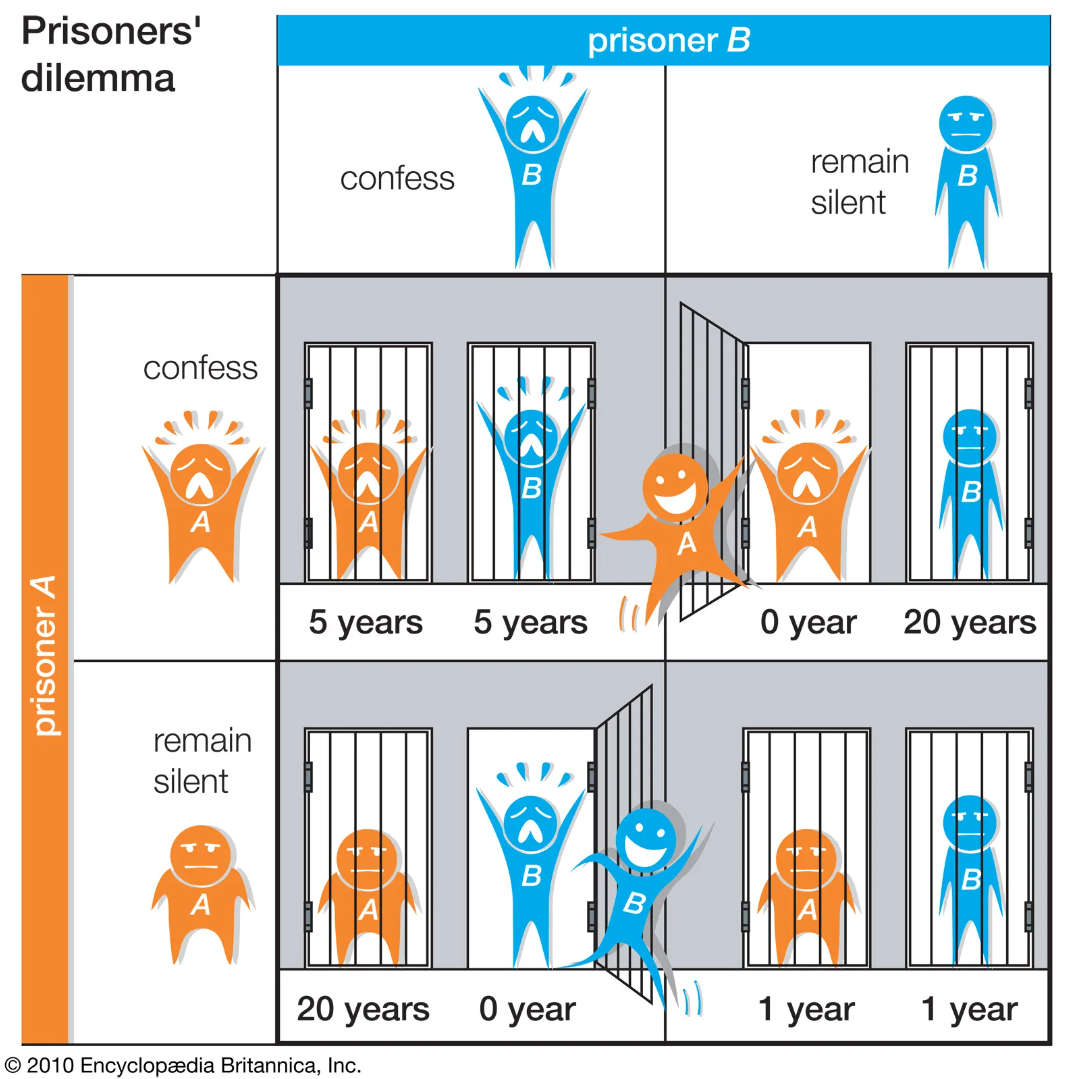
\includegraphics[height=.9\textheight]{Bin/prisonersdilemma.PNG}

\end{frame}


\begin{frame}
    \begin{center}
        \frametitle{Prisoner's Dilemma}
        \Huge
        \begin{tabular}{|c|c|c|}
            \hline
            \diagbox{P1}{P2}    & D        & C        \\
            \hline
            D                   & \(1, 1\) & \(5, 0\) \\
            \hline
            C                   & \(0, 5\) & \(3, 3\) \\
            \hline
        \end{tabular}

        \pause
        \vspace*{1cm}
        \scriptsize
        \begin{enumerate}
            \item If both players cooperate, they both get 3 points.
            \item If both players defect, they both get 1 point.
            \item If one player defects and the other cooperates, the one that
            defects gets 5 points and the one that cooperates gets 0 points.
        \end{enumerate}
    \end{center}
\end{frame}

\begin{frame}
    \begin{center}
        \frametitle{Axelrod's Tournament - 195 strategies}
        % 200 turns & 100 repetitions
        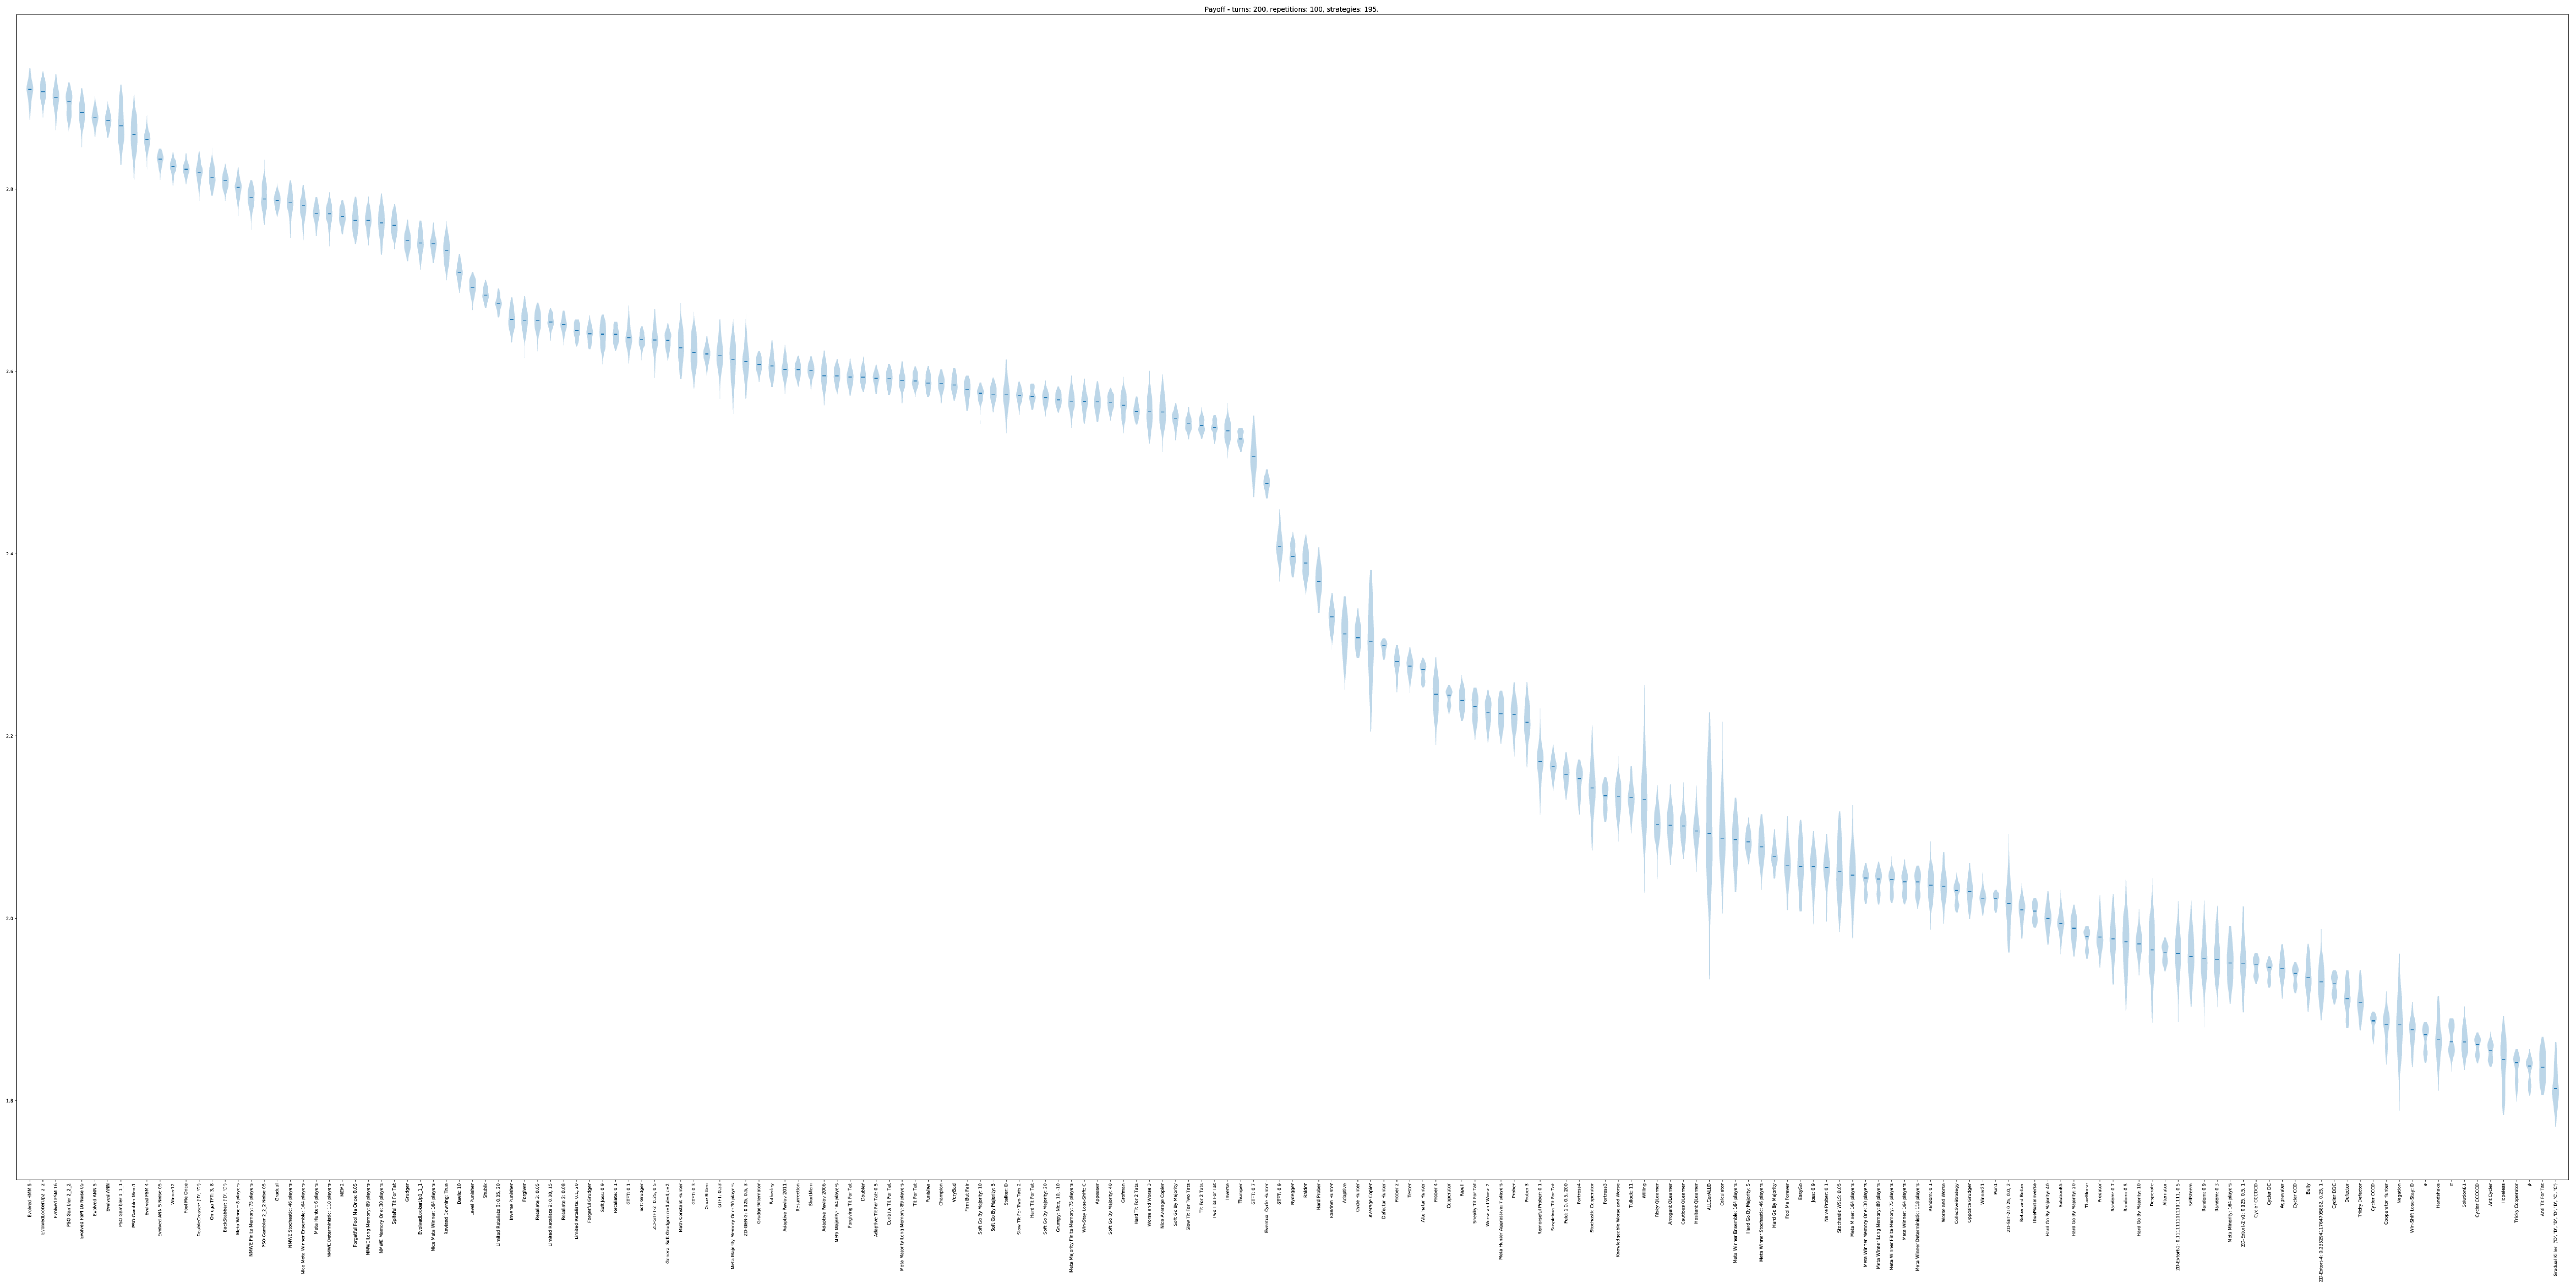
\includegraphics[width=\textwidth, trim=0 0 0 23, clip]{Bin/fulltournament.pdf}
    \end{center}
\end{frame}

\end{document}